\chapter{Progettazione e Implementazione dei Chaos Test}
In questo capitolo saranno descritti l'iter seguito per pianificare la sperimentazione, gli obiettivi prefissati al momento della progettazione e l'organizzazione dei test (Sezione 3.1).


Sarà poi esposto il processo di scelta dello strumento di Chaos Engineering usato per l'applicazione dei metodi, in supporto agli esperimenti (Sezione 3.2).

Infine, verrà descritto sinteticamente il programma creato appositamente per automatizzare la sperimentazione (Sezione 3.3).
    \section{Progettazione dei Chaos Test}
    \label{subsec:cards}
    Gli esperimenti condotti hanno seguito il formato delle \textit{Chaos Cards}, sulla base della metodologia descritta nella Sezione 2.2.3 (\textit{Steady State Hypotesis}, Metriche di verifica, metodo, \textit{Rollback}).
    
    L'ambiente della sperimentazione consiste in un'instanza di FogMon dispiegato su un \textit{testbed}, dunque il piano di \textit{Rollback} può essere ignorato a favore di un riavvio del sistema dopo la correzione della deviazione. Questa strategia infatti non comporta danni all'infrastruttura o perdita di dati significativi.
    
    
    Come anticipato nella Sezione 2.2, lo scopo di un esperimento di Chaos Engineering è scoprire le deviazioni inattese nel comportamento di un sistema, per correggerle ed aumentare la sua resilienza. Nel nostro caso, la sperimentazione di FogMon ha l'obiettivo di evidenziare, dove presenti, queste deviazioni e, possibilmente, fornire dati utili per correggerle.
    \subsection{Ipotesi di stabilità, metriche di misura}
    Per identificare le \textit{Steady State Hypotesis} di FogMon è stato svolto un periodo di monitoraggio e di analisi del prototipo. Come risultato dell'osservazione sono state formulate le seguenti ipotesi:
    \begin{itemize}
        \item H1: Il tempo massimo per la configurazione di FogMon, dopo l'avvio del calcolo della topologia, è definito e limitato a un tempo pari a 20 volte il valore del parametro \textit{time-report}, specificato nella configurazione di lancio iniziale di FogMon, con una tolleranza pari al valore di un \textit{time-report}
        \item H2: La qualità del \textit{clustering}, misurata in termini di banda e latenza, si mantiene al di sopra di una soglia prefissata (il calcolo genera un numero intero, sfruttando l'indice di Davies-Bouldin, che deve essere minore di 50)
        \item H3: I cambiamenti di stato e/o delle misure dei nodi di un gruppo, sono noti al leader entro un tempo massimo, dipendente dai parametri della configurazione di lancio iniziale di FogMon
    \end{itemize}
    Ad ognuna di queste \textit{Steady State Hypotesis} sono state affiancate delle metriche di verifica e dei metodi di sperimentazione, che riportiamo in seguito. In Figura \ref{fig:cards} è riportato uno schema di tali ipotesi con le relative metriche e i metodi utilizzati per gli esperimenti.
    \newpage    
    \begin{figure} [H]
        \begin{center}
            \begin{center}
                \begin{tabular}{|c|c|c|c|c|c|c|c|}
                    \hline
                    Steady state & Metriche di & Metodi\\
                    Hypotesis & valutazione & applicati\\
                    \hline
                    & \textbf{M1}: Organizzazione immutata  & \\
                    & per 40 propagation-time &\\
                    &&\\
                    \textbf{H1}: Tempo massimo & \textbf{M2}: Errore nelle misurazioni & Follower failure\\
                    di configurazione & inter/intra-gruppo $\leq$ 25\% & Leader failure\\
                    &&\\
                    & \textbf{M3}: Tempo massimo di &\\
                    & riconfigurazione limitato &\\
                    & dai parametri iniziali &\\
                    \hline
                    & \textbf{M1}: Se nodi = N, & \\
                    & Leader = $\lceil\sqrt{N}\rceil$ & \\
                    &&\\
                    \textbf{H2}:Qualità del & \textbf{M2}: Latenza di ogni Follower & Link failure\\
                    clustering & verso il proprio leader $\leq$ & Follower failure\\
                    & latenza verso altri leader & Leader failure\\
                    &&\\
                    & \textbf{M3}: Indice di qualità $\leq$ &\\
                    & soglia massima &\\
                    \hline
                    & \textbf{M1}: Il database del Leader  & \\
                    & di ogni gruppo elimina  & \\
                    & ogni 10 \textit{propagation-time} & Follower failure\\
                    \textbf{H3}: Diffusione dei & i dati più vecchi di 3 \textit{heartbeat} & Link failure\\
                    cambiamenti nel gruppo & & Stress test\\
                    & \textbf{M2}: L'ultimo report di ogni & \\
                    & Follower deve comparire nel &\\
                    & database del suo Leader &\\
                    &  entro due \textit{heartbeat} &\\
                    \hline
                \end{tabular}
            \end{center}
            \caption {{Le \textit{Chaos Cards} degli esperimenti con FogMon}}
            \label {fig:cards}
        \end{center}
    \end{figure}
    
    \paragraph{Tempo massimo di configurazione} 
    Questa ipotesi (H1) consiste nell'assunzione che, dopo la configurazione iniziale o in seguito all'avvio del processo di riconfigurazione, FogMon raggiunga un grado di stabilità (che definiremo come ``stabilità debole") entro un limite di tempo massimo. Si utilizzano quindi tre metriche per verificarne la validità:
    \begin{itemize}
        \item L'organizzazione dell'overlay di FogMon in Leader e Follower non cambia per 40 periodi consecutivi di comunicazione Leader-Leader (ovvero 40 volte il valore di \textit{propagation-time}, uno dei parametri di configurazione di FogMon)
        \item Tutte le misurazioni della QoS dei collegamenti e dell'hardware sono state eseguite almeno una volta in ciascun gruppo e mostrano un errore inferiore al 25\%.
        \item La riconfigurazione ha un tempo limite calcolato in base al valore di \textit{heartbeat} e di \textit{propagation-time} specificati nella configurazione iniziale di FogMon
    \end{itemize}
    Questa prima ipotesi, se verificata tramite le metriche sopracitate, indica che FogMon si è riconfigurato e ha mantenuto lo stesso overlay per un periodo sufficientemente lungo da essere considerato ``stabile". Dopo questo controllo è sensato verificare le metriche delle altre due ipotesi per capire se FogMon, in questa ``stabilità debole", funziona correttamente.
    
    
    \paragraph{Qualità del clustering} 
    Per questa ipotesi (H2) è necessario definire delle metriche in grado di verificare il rispetto del criterio di prossimità, la corretta valutazione della qualità del \textit{Clustering} e il rapporto numerico Leader-Follower, ovvero:
    \begin{itemize}
        \item I leader sono $\lceil\sqrt{N}\rceil$, dove N indica il numero di nodi monitorati da FogMon
        \item La latenza di ogni Follower verso il proprio Leader è minore della latenza verso tutti gli altri Leader
        \item L'indice di qualità calcolato dai leader ogni 5 \textit{propagation-time} (e presente nei log di output dei Leader stessi) rimane sotto una soglia massima pari a 50.
    \end{itemize}
    
    \paragraph{Diffusione dei cambiamenti nel gruppo}
    Per questa ultima ipotesi (H3), infine, sono sufficienti due metriche:
    \begin{itemize}
        \item Il Database del leader di ogni gruppo elimina ogni 10 \textit{propagation-time} i dati più vecchi di 3 \textit{heartbeat}
        \item L'ultimo report di ogni Follower deve comparire nel database del suo Leader entro due \textit{heartbeat}
    \end{itemize}
    Queste metriche, infatti, consentono di identificare delle deviazioni, qualora il leader non dovesse individuare in tempo i cambiamenti che avvengono nel proprio gruppo.
    \subsection{Metodi}
    Come descritto in nella Sezione 2.2.2, per verificare le \textit{Steady state hypotesis} si utilizzano i metodi, ovvero le modalità di test usate per causare le condizioni di ``turbolenza". Prima di descrivere quali metodi siano stati sfruttati per ogni ipotesi, ne vediamo le caratteristiche:
    \begin{itemize}
        \item \textit{Node failure}, ovvero la terminazione improvvisa di un nodo che ne simula il \textit{crash}. I \textit{Node failure} possono essere di tre tipi, in base al ruolo del nodo che terminano:
        \begin{itemize}
            \item \textit{Leader failure}, ossia la terminazione di uno o più nodi Leader,
            \item \textit{Follower failure}, ossia la terminazione di uno o più nodi Follower, oppure
            \item Una combinazione di \textit{Leader failure} e di \textit{Follower failure}, che prevede la terminazione di uno o più nodi di entrambi i ruoli.
        \end{itemize}
        
        \item \textit{Link failure}, ossia la riduzione della banda utilizzabile (nella sperimentazione, si riduce a 0.1 MB/s) e l'aumento della latenza su un collegamento tra due nodi di 500 ms
        
        \item \textit{Stress Test}, ossia una simulazione dell'aumento di uso delle risorse hardware di un nodo (nella sperimentazione, si aumenta l'uso della CPU fino a 7 core sugli 8 disponibili e della RAM di oltre 500MB)
    \end{itemize}
    \paragraph{Metodi per H1}
    
    Per verificare la prima ipotesi sono stati utilizzati dei test di tipo \textit{Node failure} (\textit{Leader failure}, \textit{Follower failure} e la loro combinazione). 
    \begin{itemize}
        \item Il \textit{Leader failure} consente di abbassare il numero dei Leader al di sotto della soglia prevista di $\sqrt{N}$, innescando il ricalcolo della topologia.
        \item I \textit{Follower failure}, similmente, se in numero sufficientemente elevato possono ridurre il numero di Follower e causare lo stesso processo descritto al punto precedente.
    \end{itemize}  Questi metodi dunque causano la riorganizzazione dell'overlay di FogMon, garantendo così la possibilità di monitorare la fase di riconfigurazione e identificarne eventuali deviazioni.
    
    
    \paragraph{Metodi per H2}
    
    La verifica della seconda ipotesi consiste nell'applicazione dei metodi di \textit{node failure} e \textit{link failure}.
    \begin{itemize}
        \item Un esperimento con \textit{node failure}, come già accennato per H1, può innescare la riconfigurazione dell'overlay di FogMon, permettendo di verificare il corretto funzionamentotramite la prima metrica della seconda ipotesi (ovvero la condizione per cui se la rete è composta da N nodi, i Leader devono essere $\sqrt{N}$).
        
        \item  Effettuando i \emph{Link failure}, invece, si causa un cambiamento delle condizioni di rete che dovrebbe portare al cambio di leader per i nodi coinvolti. Più in particolare, i Follower interessati devono cambiare leader se le misurazioni indicano che quello attuale non è più il migliore in termini di latenza. Tale esperimento permette dunque di verificare la qualità del \textit{clustering}, misurata dalle ultime due metriche della seconda ipotesi.
    \end{itemize}
    Più in dettaglio, i \emph{Link failure} causano un peggioramento della QoS di rete, che porta a un peggioramento della qualità del \textit{clustering}. Il calcolo dell'indice di qualità, a questo punto, avrà come risultato un indice al di sopra della soglia massima e dovrebbe portare al ricalcolo della topologia. Se questo non avviene, siamo di fronte a una deviazione.
    
    
    \paragraph{Metodi per H3}
    
    Infine, per la verifica della terza ipotesi, sulla base delle metriche scelte, si sfruttano \textit{Link failure}, \textit{Follower failure} e \textit{Stress test}.
    \begin {itemize}
        \item I \textit{Follower failure} consentono di verificare se un Leader, dopo al massimo 10 \textit{propagation-time}, rimuove i Follower disconnessi da più di 3 \textit{heartbeat}
        \item I \textit{Link failure} permettono di verificare la velocità con cui un peggioramento delle condizioni di rete si propaga all'interno del gruppo di appartenenza dei nodi coinvolti
        \item Lo \textit{stress test}, infine, verifica la velocità con cui l'aumento di utilizzo delle risorse di un nodo viene segnalato all'interno del gruppo di appartenenza del nodo stesso.
    \end {itemize}
    \section{Implementazione degli esperimenti}
    Per automatizzare le operazioni di applicazione dei metodi, della raccolta delle risposte e del monitoraggio dell'attività di FogMon, è stato scelto uno strumento di Chaos Engineering che consenta di svolgere le operazioni descritte (Sezione 3.2.1) ed è stato realizzato un programma (Sezione 3.2.2) che permetta di sfruttare questo strumento come supporto per l'iniezione dei fallimenti in FogMon.
        \subsection{Scelta dello strumento Pumba}
        \label{subsec:pumba}
        Per prima cosa, si rende necessario trovare uno strumento per attuare i metodi descritti nella Sezione 3.1. A questo scopo si prestano numerosi mezzi ed è quindi necessario discernere quali siano i più adatti al software da testare.
        Di seguito i criteri di valutazione degli strumenti valutati:
        \begin {itemize}
            \item Supporto alle applicazioni containerizzate: Fogmon è un prototipo distribuito su container Docker, pertanto lo strumento deve avere la possibilità di operare su un'applicazione containerizzata. Verrà data la preferenza agli strumenti già orientati all'uso con Docker.
            
            \item Bassi requisiti hardware: FogMon opera in ambiente Fog, quindi la sperimentazione deve avere il minore impatto possibile sull'utilizzo delle risorse dei nodi.  Pertanto gli strumenti con requisiti inferiori ai 512 MB di memoria RAM verranno privilegiati.
            
            \item Assistenza e supporto validi: sarà considerata, ai fini della scelta, anche la quantità di materiale informativo sul software, l'assistenza da parte degli sviluppatori e l'aiuto da parte della \textit{community}, tutti aspetti che facilitano l'integrazione e l'uso dello strumento.
            
            \item Licenza gratuita: gli strumenti che consentano di effettuare i test di Chaos Engineering su FogMon con licenza gratuita hanno la priorità.
            
            \item Funzionalità: lo strumento scelto deve fornire la possibilità di intervenire con i metodi descritti nella Sezione 2.2.2. Pertanto, deve garantire la possibilità di causare \textit{Node failure}, \textit{Link failure} e \textit{Stress Test}
        \end {itemize}
        Lo studio effettuato ha visto la comparazione di vari strumenti pubblicamente disponibili, ideati per svolgere tale compito. Di seguito si riportano i principali:
        \begin{itemize}
        
            \item Chaos Monkey \cite{Netflix}: Uno dei primi \textit{toolkit} di Chaos Engineering, creato da Netflix. Tutt’ora aggiornato regolarmente, fornisce una suite completa per la sperimentazione e l’automatizzazione degli esperimenti di chaos engineering su architetture distribuite. È costantemente aggiornato e gode di una \textit{community} attiva, tuttavia è stato scartato per le ingenti risorse hardware necessarie per l’integrazione (richiede vari GB di RAM), oltre alla necessità di usare Kubernetes anzichè Docker. 
            
            
            \item Chaos toolkit \cite{chaostoolkit}: È una suite di Chaos Engineering ampiamente usata, gode di una documentazione estesa per la distribuzione su Kubernetes sebbene sia utilizzabile anche con Docker; riceve meno aggiornamenti di Chaos Monkey, pur godendo delle stesse funzionalità. Non presenta requisiti hardware particolarmente elevati (pochi KB di RAM) ed ha possibilità di integrazione con Docker, ma l'assistenza da parte degli sviluppatori sembra praticamente assente, così come la \textit{community}. 
            
            \item Gremlin \cite{gremlin}: Fornisce agli utenti un insieme completo e affidabile di strumenti; è utilizzato da più di 8 anni e presenta una \textit{community} attiva, con cui interagire facilmente; in più, ha una buona integrazione con Docker. Il piano gratuito, tuttavia, impone dei limiti sull'uso (riducendo il numero massimo di interventi mensili), rendendolo di fatto insufficiente a svolgere pienamente il compito richiesto.
            
            
            \item Pumba \cite{pumba}: Permette di iniettare fallimenti sui nodi e sulla rete, su licenza gratuita. È costantemente aggiornato, dispone di una \textit{community} molto attiva, ha un'ottima compatibilità con Docker (fornendo sia un'immagine ad hoc su cui poter effettuare la distribuzione del servizio, sia un eseguibile da integrare nei propri container) e presenta dei requisiti hardware molto bassi (pochi KB di RAM).
            
            \item Chaosblade \cite{blade}: \textit{Open source}, richiede risorse limitate ed è compatibile con Docker e Kubernetes. Non è, tuttavia, ancora alla versione completa, l'assistenza da parte degli sviluppatori è limitata alla possibilità di contatto via e-mail o su GitHub e la \textit{community} è molto meno attiva delle controparti. 
            
            \item Hystrix \cite{hystrix}: strumento di supporto a Chaos Monkey, in quanto sviluppato da Netflix parallelamente alla \textit{Simian Army}. Non è usabile singolarmente; gode di un'ottima assistenza da parte degli sviluppatori (come Chaos Monkey) ma presenta dei requisiti hardware alti (oltre il GB di RAM) e funziona esclusivamente su Kuberntes. Non è, perciò, adatto per la sperimentazione su Fogmon. 
        \end{itemize}
        Nella Tabella \ref{tab:pumba} riportiamo sinteticamente un confronto tra questi strumenti:
        \begin{table}
        \begin{center}
            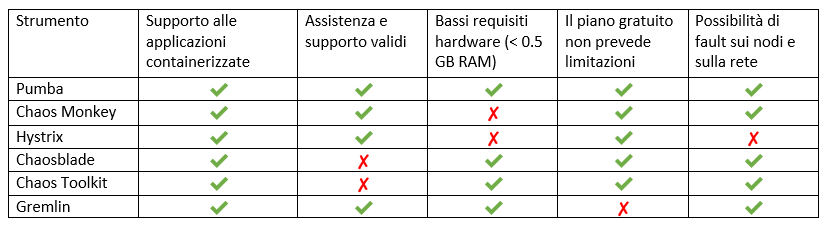
\includegraphics[width=14cm, height=4cm]{images/tabella.png}
            \caption {Pumba presenta tutti i requisiti più importanti}
            \label {tab:pumba}
        \end{center}
        \end{table}
        vista la possibilità di usufruire di una suite completa di interventi in modo gratuito, i requisiti hardware praticamente trascurabili, la distribuzione con licenza Apache 2.0 \cite{Apache} e l'esistenza di un eseguibile scaricabile e usabile direttamente sui nodi che eseguono i container Docker, la scelta finale è stata Pumba. 
        
        Pumba permette di effettuare le seguenti operazioni: 
        \begin{itemize}
            \item \textit{Kill}: consente di terminare un container, specificando il segnale desiderato da inviare al processo nel container.
            
            \item \textit{Pause}: permette di sospendere temporaneamente il processo all'interno del container, specificando la possibilità di riavvio automatico
            
            \item \textit{Netem}: permette di utilizzare gli strumenti di \textit{Traffic Control} (tc) \cite{tc} tramite i comandi:
            \begin{itemize}
                \item \textit{Delay}: aumenta la latenza di tutti i pacchetti in uscita dai container specificati
                \item \textit{Loss}: aggiunge una probabilità (impostabile) di perdita di pacchetti
                \item\textit{ Rate}: limita la banda per tutti i pacchetti in uscita dai container specificati
                \item \textit{Duplicate}: aggiunge una probabilità (impostabile) di duplicazione di pacchetti
                \item \textit{Corrupt}: aggiunge una probabilità (impostabile) di corruzione di pacchetti
            \end{itemize}
            
            \item \textit{Stress}: simula un aumento di utilizzo delle risorse indicate dei container specificati
        \end{itemize}
       Ogni comando possiede una collezione di flag e attributi per specificare la durata, gli intervalli e le modalità di applicazione dei metodi (indicando, ad esempio, l’interfaccia di rete per \textit{netem} o la componente nel caso di stress).\\\\Alcuni esempi di comandi vengono riportati di seguito:\\\\
        \texttt{pumba netem --duration 5m delay --time 3000 mydb} (delay di 3 secondi su tutti i pacchetti in uscita sull’interfaccia default del container mydb)\\\\
        \texttt{pumba netem --duration 5m corrupt --percent 10 mydb} (corruzione del 10\% dei pacchetti in uscita dal container mydb per 5 minuti) \\\\
        \texttt{pumba stress --duration 5m CPU--load10 mydb} (stress della CPU con carico al 10\% del container mydb per 5 minuti)\\\\
        \texttt{pumba --random --interval 1s kill --signal SIGKILL} (invio di SIGINT a container selezionati pseudorandomicamente, con intervallo di un secondo)\\
    
        \subsection{Automazione dei test: FogMonK}
        \label{subsec:FogMonK}
        FogMonK è un programma realizzato in Java, che si pone l’obiettivo di automatizzare l'esecuzione degli esperimenti di Chaos tramite Pumba, monitorare lo stato del sistema e raccogliere i dati di FogMon, senza la necessità di un utente che osservi attivamente il processo.
        
        FogMonK interopera con FogMonEye e, pertanto, sfrutta la creazione di “momenti” (le fasi di un esperimento già descritte in 2.1.4) e sul controllo dei cambiamenti del sistema tra questi ultimi. Più precisamente, FogMonK non si limita a effettuare delle “fotografie” del sistema prima e dopo ogni fase, ma cerca di identificare le cause delle possibili deviazioni.
        
        In base all'esperimento da eseguire, l'utente può specificare un insieme di parametri come input: 
        \begin{itemize}
            \item Tipo di test (\textit{kill, netem, stress}) 
            
            \item Ruolo dei nodi a cui applicare il test (Leader/Follower oppure i nodi specifici, da indicare con il nome del nodo) 
            
            \item Percentuale dei nodi a cui applicare il test, chiaramente non utilizzata qualora vengano indicati i nodi specifici su cui applicare i metodi 
            
            \item Tempo limite per la stabilità 
            
            \item Riavvio automatico in caso di \textit{Node failure} dei nodi 
        \end{itemize}
        Oltre a questi parametri generici troviamo quelli riservati esclusivamente ad alcuni test: 
        \begin{itemize}
            \item In caso di \textit{kill}, il lasso di tempo da attendere tra l’abbattimento di un nodo e quello del successivo 
            
            \item In caso di \textit{netem}, la percentuale di perdita dei pacchetti, la latenza da aggiungere ai nodi o l’utilizzo di banda, in percentuale 
            
            \item In caso di \textit{stress}, la componente da andare a sottoporre a sforzo e la percentuale di utilizzo desiderata 
        \end{itemize}
        La configurazione di input sfrutta un file in formato JSON per ragioni di manutenibilità del codice e facilità nell’implementare nuovi parametri e nuove funzioni.
        
        Per quanto riguarda l'output, FogMonK restituisce le seguenti informazioni al termine di un esperimento: 
        \begin{itemize}
            \item Id di sessione di FogMonEye (ovvero un numero identificativo dell'esperimento)
            
            \item Id dell’esperimento 
            
            \item Sommario dell’input 
            
            \item Elenco dei nodi e delle loro informazioni 
                \begin{itemize}
                \item Nome 
                
                \item Stato prima dell’esperimento (\textit{alive/killed}) 
                
                \item Gruppo di appartenenza iniziale 
                
                \item Ruolo iniziale 
                
                \item Test effettuato 
                
                \item Gruppo di appartenenza finale 
                
                \item Ruolo finale 
                
                \item Stato dopo l’esperimento 
                \end {itemize}
            
            \item Tempo di inizio esperimento (gg/mm/aa, h:m:s:ms) 
            
            \item Tempo di fine esperimento 
            
            \item Tempo di stabilità 
            
            \item Errore sulle misurazioni di latenza e banda 
            
            \item Sommario di verifica delle ipotesi. Questo sommario consiste nell'elenco delle metriche verificate nell'esperimento e nel risultato di tale verifica, pertanto è di fondamentale importanza per comprendere se la seconda stabilità sia stata raggiunta e se le metriche di verifica delle ipotesi rientrino nei valori corretti
            
            \item Superamento del test 
        \end{itemize}
        L'output riesce a rappresentare un momento (inteso come l'insieme degli eventi che vanno dalla stabilità iniziale a quella successiva all'applicazione del metodo), integrando quindi il controllo delle eventuali deviazioni e identificando comportamenti o arresti anomali. Il report di tutti i nodi serve a facilitare l'analisi che l'utente esegue al termine dell'esperimento. Il risultato avrà un aspetto simile alla Figura \ref{fig:output}.
        \begin{figure}
            \begin{center}
                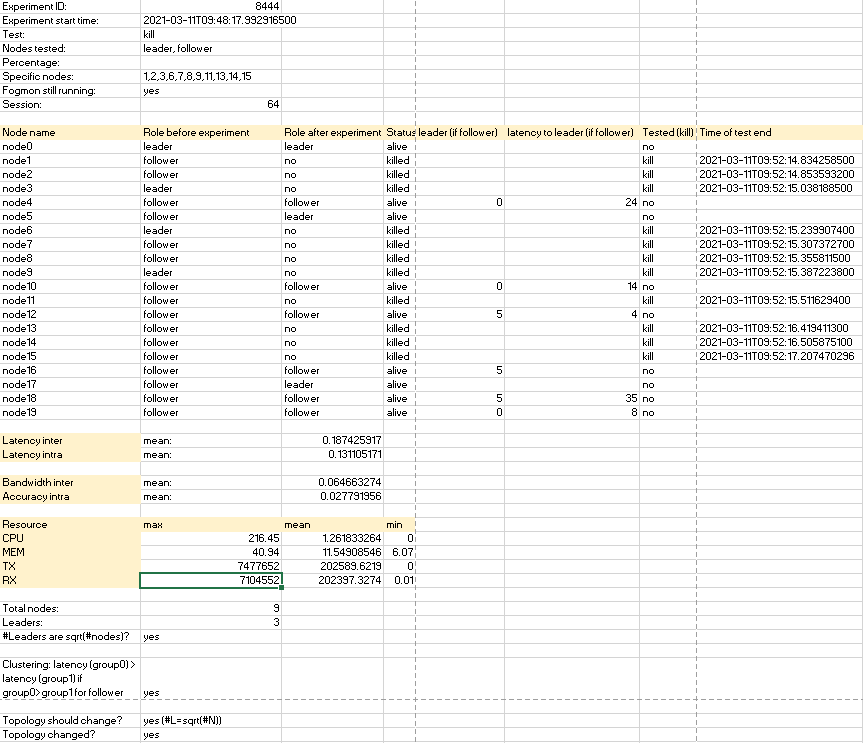
\includegraphics[width=13cm, height=13cm]{images/out.png}
                \caption {Un esempio di output di FogMonK}
                \label{fig:output}
            \end{center}
        \end{figure}

        \paragraph{Fasi di sperimentazione con FogMonK}\mbox{}\newline
        Un esperimento svolto con FogMonK segue l'iter descritto al Capitolo 2.2. Dopo l'avvio del testbed e di FogMon, le fasi sono:
        \begin{itemize}
            \item Verifica della prima stabilità e controllo delle metriche delle \textit{Steady State Hypotesis}. Se le metriche non rientrano nello spettro dei valori accettabili, l'esperimento viene concluso, identificando il problema
            \item Se FogMon raggiunge la prima stabilità, FogMonK sfrutta Pumba per applicare il metodo previsto nella configurazione dell'esperimento
            \item FogMonK attende fino alla validità dell'ipotesi H1 descritta nella Sezione 3.1. Se questa non viene raggiunta, si identifica la deviazione nel report di output
            \item Anche se l'ipotesi H1 viene raggiunta, ma le metriche di H2 e H3 non rientrano nello spettro dei valori accettabili, si rileva una deviazione
            \item Se tutte le \textit{Steady State Hypotesis} sono verificate, l'esperimento termina senza deviazioni identificate
        \end{itemize}
        Ricordiamo che le prime due metriche dell'ipotesi H1 sono:
        \begin{itemize}
            \item L'organizzazione dell'overlay di FogMon in Leader e Follower non cambia per 40 periodi consecutivi di comunicazione Leader-Leader (ovvero 40 volte il valore di \textit{propagation-time}, uno dei parametri di configurazione di FogMon)
            \item Tutte le misurazioni della QoS dei collegamenti e dell'hardware sono state eseguite almeno una volta in ciascun gruppo e mostrano un errore inferiore al 25\%.
        \end{itemize}
        La verifica di H1 sfrutta, per queste prime due metriche, i servizi offerti da FogMonEye. Per tutte le altre verifiche, FogMonK controlla se le metriche descritte nella Sezione 3.1 rientrano nello spettro dei valori accettabili tramite controlli sui file di log dei nodi, interrogazioni ai database e monitoraggio dell'uso delle risorse.
        
        FogMonK invoca comandi Pumba per l'applicazione di tutti i metodi. In particolare:
        \begin{itemize}
            \item Per il metodo \textit{Node failure}, FogMonK lancia l'esecuzione del comando \textit{pumba kill} sui nodi destinati al fallimento
            \item Per il metodo \textit{Link failure}, FogMonK usa il comando \textit{pumba netem} sui nodi collegati dal \textit{link}, specificando l'interfaccia di rete di ciascun nodo
            \item Per il metodo \textit{Stress test}, FogMonK lancia il comando \textit{pumba stress} sui nodi da sottoporre all'esperimento
        \end{itemize}
        I comandi addizionali di Pumba vengono scelti da FogMonK in base alla configurazione di input dell'utente.
        
        \paragraph{Principali classi di FogMonK}
        In Figura \ref{fig:classes} vediamo un diagramma delle classi principali di FogMonK. Di queste, nei successivi paragrafi saranno presentate sinteticamente le tre più importanti per lo svolgimento delle funzioni di FogMonK.
                
        \begin{figure}[H]
            \begin{center}
                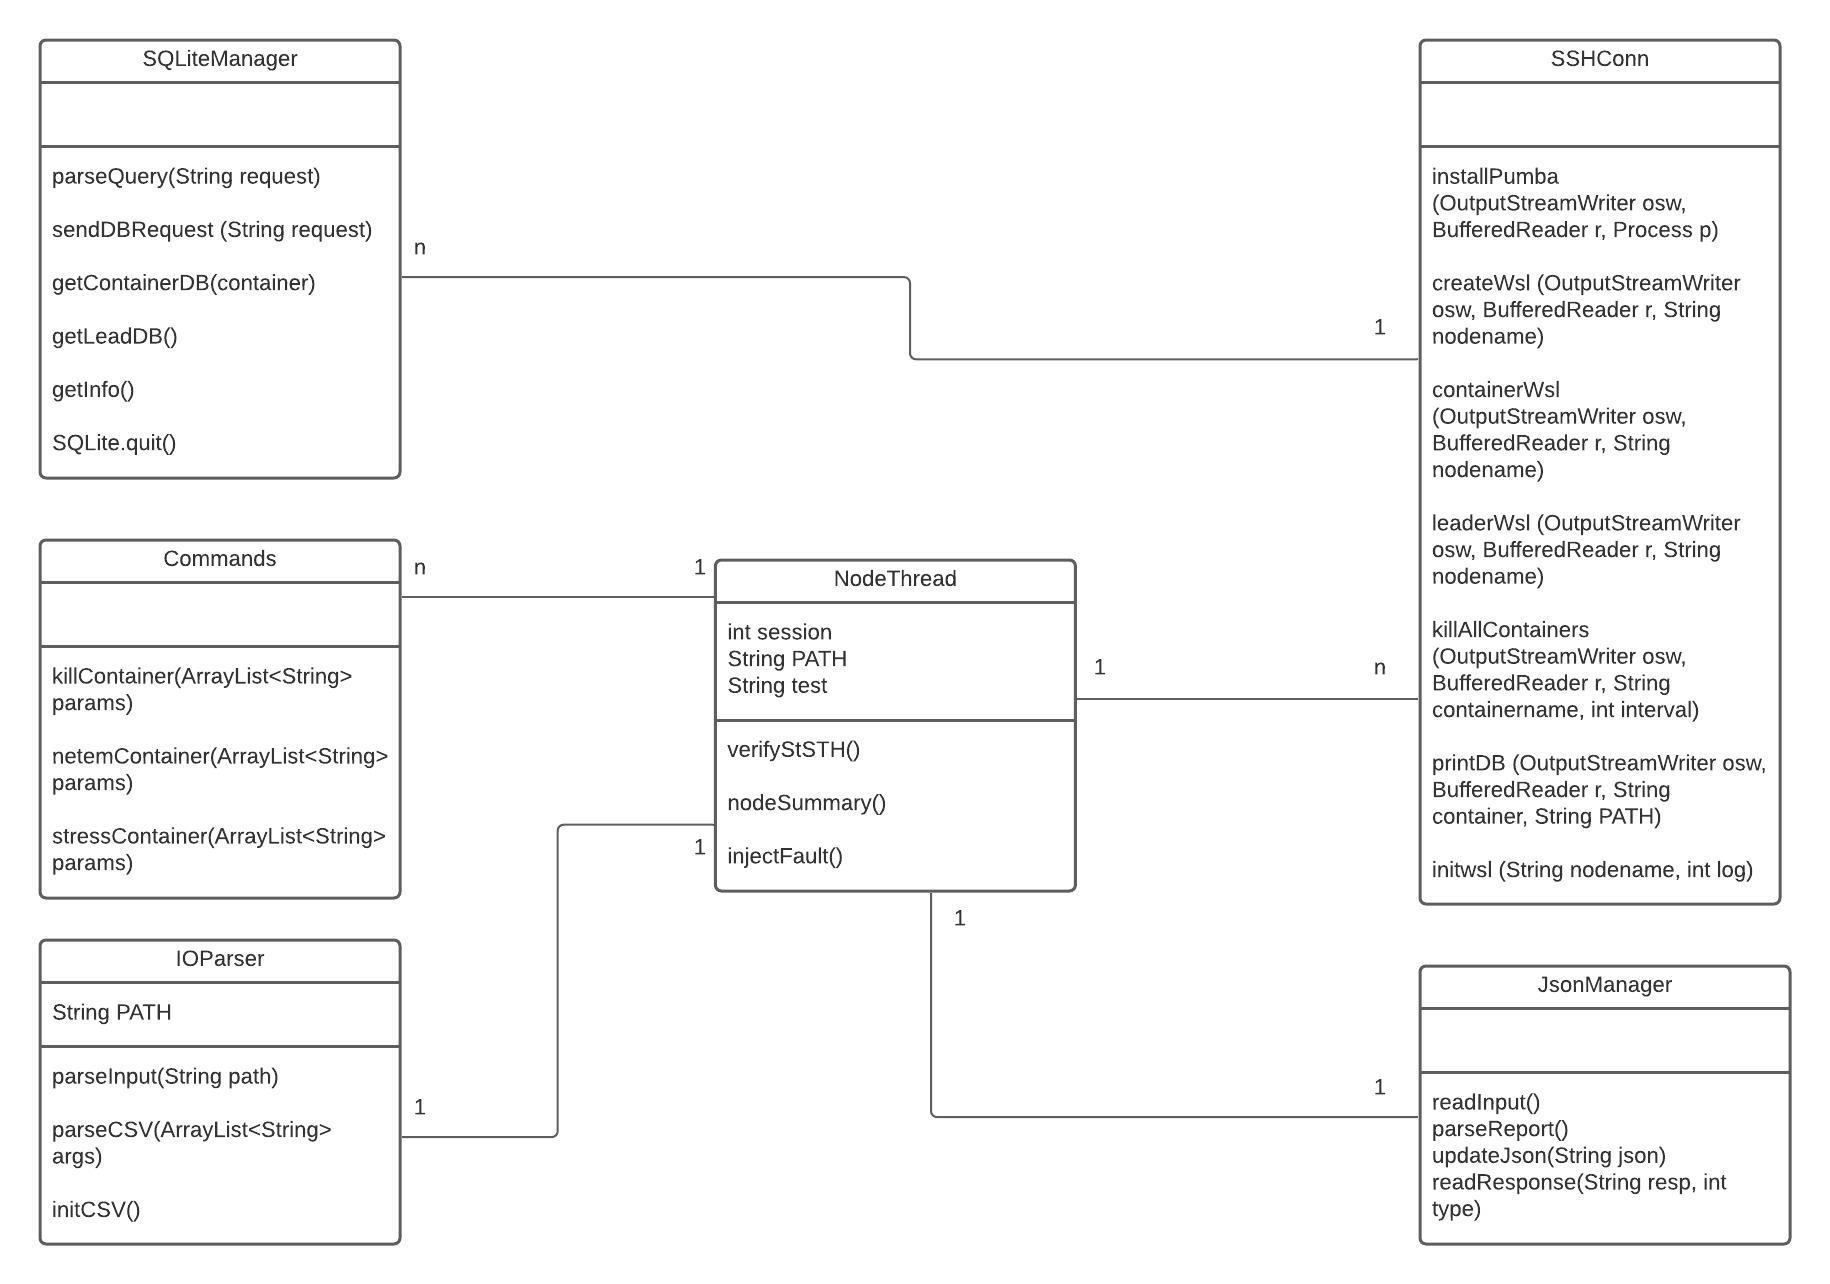
\includegraphics[width=13cm, height=10cm]{images/diag.classi.tesi.jpeg}
                \caption {Organizzazione in classi di FogMonK}
                \label{fig:classes}
            \end{center}
        \end{figure}
        
        \paragraph{La classe JsonManager}\mbox{}\newline
        Come già menzionato, il formato dell’input sfrutta JSON; ne vediamo un esempio nella figura \ref{fig:json}.
        \begin{figure}
            \begin{center}
                \begin{lstlisting}

                    files = ["in"] 
                    name_override = "jsoninput" 
                    data_format = "json" 
                    
                    {
                    "type": "kill", 
                    "nodetype": "leader", 
                    "specnodes": [], 
                    "timelimit": 600, 
                    "percent": 80, 
                    "restartoncrash": "false", 
                    "killtimewait": , 
                    "netemlaten": , 
                    "netemband": , 
                    "stresscomp": 
                    "connum": , 
                    }
                    
                \end{lstlisting}
                \caption {Parametri di input di un esperimento di tipo \textit{Leader failure}}
                \label{fig:json}
            \end{center}
        \end{figure}
        
        Per la raccolta dei dati, la gestione dei dati da scambiare con FogMonEye e, più in generale, per le conversioni di stringhe da e verso JSON, FogMonK contiene la classe JsonParser, di cui riportiamo i metodi più usati e importanti:
        \begin{itemize}
            \item \texttt{readInput()}: si occupa di leggere i dati di ingresso forniti dall'utente nel file JSON. Tali dati verranno poi comunicati al thread principale, incaricato di variare i comandi da lanciare in base ai parametri selezionati
            \item \texttt{parseReport()}: crea una stringa JSON da inviare successivamente a FogMonEye, per aggiornarlo di cambiamenti avvenuti nella topologia di rete (disconnessione di nodi, eliminazione di link, etc)
            \item \texttt{updateJson(String json)}: aggiorna il file di specifica contenente le informazioni sulla rete, viene invocato in caso di connessione/disconnessione di nodi o di creazione/distruzione di link
            \item \texttt{readResponse(String resp, int type)}: converte i dati ottenuti dalle risposte di FogMonEye. Il parametro type indica di che tipo di risposta si tratti (richiesta dei dati di \textit{accuracy} e \textit{performance}, richiesta di \textit{footprint}, conferma della creazione del momento, etc)
        \end{itemize}
        Per evitare di creare un gestore JSON personalizzato, si fa uso delle librerie Google Gson \cite{gson} che semplificano il processo di conversione da \textit{Json Object} a stringa, ma si rivelano molto comode anche nel processo inverso, a patto di avere una classe pronta a incapsulare i dati contenuti nella stringa JSON.
        
        Anche i file contenenti le informazioni sulla topologia e sulle condizioni dei singoli nodi (\textit{spec}) sfruttano la notazione JSON e, con essi, anche i report da inviare a FogMonEye (contenenti le informazioni sulle variazioni della topologia di rete monitorata da FogMon); l’elaborazione di questi file, al crescere del numero di nodi, mostra dei limiti in fatto di efficienza. In futuro, se la dimensione dei dati dovesse aumentare, andrebbe considerata la possibilità di variarne la modalità di rappresentazione in favore di una più efficiente e veloce(YAML XML).
        \paragraph{La classe SSHConn}\mbox{}\newline
        Per il monitoraggio e l'applicazione dei metodi in FogMon, l'installazione di Pumba e la verifica delle ipotesi FogMonK si connette direttamente ai nodi su cui FogMon è distribuito.
        
        Vista la possibilità che Fed4Fire offre di connettersi in SSH ai nodi degli esperimenti istanziati sui loro \textit{testbed}, la soluzione adottata è proprio la creazione di Thread che si occupino di instaurare una connessione con il nodo e di riportare fedelmente ogni dettaglio dell’interazione su dei log dedicati.
        
        Anziché sfruttare librerie di terze parti per le connessioni SSH, FogMonK genera dei terminali usando le chiavi e gli id RSA memorizzati tramite gli strumenti forniti da Jfed; pertanto, per instaurare una connessione è sufficiente lanciare un terminale con il comando “ssh -F ssh-config -I id\_rsa [user]@[nodename]” e specificare un OutputStreamWriter e un InputStreamReader per la comunicazione tra FogMonK e il terminale appena creato.
        
        Per ogni nodo, come menzionato, possono essere instaurate più connessioni, in dettaglio: 
        \begin{itemize}
            \item Una per il monitoraggio del database: 
            FogMonK deve poter controllare i dati del database di ogni nodo per verificarne l’integrità 
            
            \item Una per il monitoraggio del log di FogMon: 
            FogMonK accede ai log di ogni nodo per verificare i possibili errori nella comunicazione tra FogMon e FogMonEye, i \textit{node failure} inattesi, la valutazione che FogMon stesso effettua della qualità del servizio (se insoddisfacente può portare a una riconfigurazione) e la frequenza delle rilevazioni sulla latenza e sulla banda 
            
            \item Una per il lancio di comandi e la raccolta delle risposte: 
            ogni comando, compresi quelli per l'applicazione dei metodi, ha bisogno di un terminale dedicato per la raccolta e l’analisi delle risposte 
             
            \item Una al primo avvio dell’esperimento, per installare Pumba in caso non sia già presente sulla macchina: 
            FogMonK verifica la presenza di Pumba tramite una ricerca nella cartella di installazione predefinita; se assente, lo installa.
        \end{itemize}
        Ogni volta che FogMonK necessita di una connessione, la crea tramite la classe SSHConn. Tutte le connessioni vengono terminate quando esauriscono il loro ruolo, per evitare di dover gestire troppi stream di input e output e rallentare l'esecuzione di FogMonK.
        \paragraph{La classe SQLiteManager}\mbox{}\newline
        La classe SQLiteManager si occupa di incapsulare comandi SQLite3 per i terminali che realizzano le connessioni, di interpretare le risposte delle interrogazioni ai \textit{DataBase} di FogMon e di decapsularle per convertirle in dati utili a FogMonK.
        
        Trattandosi di un accesso ``esterno" ai database, SQLiteManager fornisce un metodo di gestione degli errori di lettura del DB, che possono verificarsi nel caso in cui esso sia in uso da FogMon al momento dell'accesso da parte di FogMonK. In tal caso, FogMonK ripeterà l'interrogazione dopo un intervallo prestabilito. Tra i metodi principali troviamo:
        \begin{itemize}
            \item \texttt{parseQuery(String request)}: esegue la query richiesta in un database precedentemente aperto e salva la risposta nella cartella predefinita
            \item \texttt{sendDBRequest (String request)}: richiede l'accesso a un database per poterlo utilizzare
            \item \texttt{getContainerDB(String container)}: dopo aver richiesto l'accesso, apre il database per accedere ai dati con query
            \item \texttt{getLeadDB()}: apre il database dei nodi leader in cui è invocato
            \item \texttt{getInfo(String op)}: stampa le informazioni richieste in base al parametro \textit{op} con cui è invocato
            \item \texttt {SQLite.quit()}: chiude il database in uso e la console SQLite3 che era aperta nel terminale
        \end{itemize}










